\chapter{Implementation}
\label{cha:implementation}

The previous chapter explained the central concept of the work. The current chapter covers technical implementation details and addresses the following questions:

\begin{itemize}
  \item development tools, environments, frameworks and a programming language used for implementation.
  \item The sequential stages of the data processing pipeline with the set of techniques and their implementation.
  \item The application for interactive data visualization in a low-dimensional space. The application wrappers around the data science pipeline.
  \item The evaluation of the results of the branched pipeline and its implementation.
  \item Deliverables of the thesis.
\end{itemize}

\section{Implementation environment and programming language}
The basic data science pipeline~\ref{Overall data science pipeline for user segmentation} as well as the demo application~\ref{Demo application} are written in Python 3.7. Python is an interpreted, high-level, general-purpose programming language. It is developed under OSI-approved open source license. Numerous Python community developed a variety of libraries for almost any purpose. The language is equally good for building web server applications and manipulations with raw data, analysis and visualization. These were the decisive factors for choosing this particular programming language for the implementation part of the current work. The auxiliary packages along with the purposes of use in the present work are listed in the~\autoref{tab:tab3}.

The proposed data science pipeline is developed and submitted as a set of Jupyter Notebooks. Jupyter Notebook is an open-source web application commonly used for scientific computing and data science. It is suitable for working with live code, equations, visualizations and explanatory text all in one. It was intentionally developed for data cleaning and transformation, numerical simulation, statistical modelling, machine learning and other data science specific purposes~\cite{Jupyter_Notebook}. Jupyter Notebook was developed as a part of the open-source Jupyter project for interactive computing across different programming languages. It released under the liberal terms of the modified BSD license~\footnote{
\textbf{BSD license} is a class of simple and liberal licenses for computer software with two main restrictions: (1) one should not claim that they wrote the software if they did not write it and (2) one should not sue the developer if the software does not function as expected or as desired. Source: http://www.linfo.org/bsdlicense.html}.

PyCharm is an open-source cross-platform integrated development environment which supports web development in Python. It has plenty of features for writing code such as code analysis, a graphical debugger, an integrated unit tester. PyCharm Community Edition is distributed under Apache 2 license~\footnote{\textbf{Apache license} is a permissive free software license written by the Apache Software Foundation. Source: http://www.apache.org/licenses/}.

\begin{table}
\begin{center}
\begin{tabular}{ | m{0.7em} | m{1.7cm} | m{1.5cm} | m{11cm} |} 
\hline
\textbf{\#} & \textbf{package} & \textbf{version} & \textbf{purpose of usage} \\ 
\hline
1 & pandas & 0.23.4 & Data preprocessing and manipulations with data frames \\
\hline
2 & numpy & 1.16.4 & Work with multi-dimensional vectors \\
\hline
3 & datetime & 3.7 & Dates converting, transactions' timestamps processing \\
\hline
4 & random & 3.7 & Incorporation of time classes into semi-random walks in case of multi-edges \\ 
\hline
5 & networkx & 2.2 & Graph representation of financial transaction networks \\
\hline
6 & itertools & 3.7 & Generation of modified sequences by merging semi-random walks and additional information components \\
\hline
7 & matplotlib & 3.1.1 & 2d visualisation \\
\hline
8 & mplot3d & 3.1.1 & 3d visualisation \\
\hline
9 & scikit-learn & 0.21.2 & Clustering validation metrics  \\
\hline
10 & jqmcvi & 1.0 & Dunn clustering validation metric  \\
\hline
10 & math & 3.7 & Mathematical operations (sqrt) \\
\hline
11 & scipy & 1.2.1 & Spatial distances in a metric space \\
\hline
\end{tabular}
\caption {Python packages used for the implementation of the data science pipeline and demo application (compatible with Python 3.7 version).}
\label{tab:tab3}
\end{center}
\end {table}

\section{Overall data science pipeline for user segmentation}
\label{Overall data science pipeline for user segmentation}
This section covers each phase of the technical implementation of the developed pipeline. All stages are developed as a Python script. The sequential stages conceptually have been described in the previous chapter on the~\autoref{fig:Fig28}. This section will discuss in detail how they are implemented including data preparation, processing and evaluation phases.

The data preparation in general case includes converting a financial transaction data to a data set of $N$ transactions each of them described by "Source" - a user who initiates a transaction, "Target" - a user who received a transaction and "Timestamp" - when the transaction has been transferred. The next crucial step is to convert "Timestamp" feature to the time classes. To come up with the relevant time classes splitting, it is necessary to follow two rules: 
\begin{enumerate}
    \item The number of time classes should not be too large. As the goal is to come with the clusters of similar users, a time class should span enough users who were active during a certain time period.
    \item The number of time classes should not be too low. If too many users would be active during the same period, they will be placed close to each other in a metric space making too large indistinguishable clusters of similar users. 
\end{enumerate}
To choose the optimal number of time classes, some forehand time analysis is required. It may need to convert "Timestamp" values to datetime format to explore transaction distribution over time. In general, the time classes splitting is an input data set-dependent procedure.

The data processing phase consists of network embedding learning, dimensionality reduction and cluster analysis stages (\autoref{fig:Fig28}). The stages are implemented consequently within one Python script. The script exploits several existing frameworks chained together. These frameworks along with their original sources are listed in the~\autoref{tab:tab4}. The Node2vec framework is used for generating semi-random walks from a network. Then the semi-random walks are transformed to ordered sequences according to imputation strategies from~\ref{Time component} and~\ref{Global structural component}. The Word2vec from the gensim.models package provides a fast realization of the skip-gram model which allows learning features from ordered sequences. The next stage takes the output of skip-gram model as an input for further dimensionality reduction. The UMAP, t-SNE, and PCA frameworks produces low-dimensional embeddings from arbitrary dimensional data. This step facilitates the future cluster analysis by reducing the negative effects of the "curse of dimensionality". The next stage groups the outputting embeddings into clusters. Two frameworks HDBSCAN and k-means serve this purpose and produce sets of users split into clusters.
\begin{table}
\begin{center}
\begin{tabular}{ | m{0.7em} | m{2cm} | m{3.7cm} | m{1.5cm}| m{7cm} |} 
\hline
\textbf{\#} & \textbf{framework} & \textbf{software package} & \textbf{version} & \textbf{source} \\ 
\hline
1 & Node2vec & node2vec & 0.2.1 & https://github.com/eliorc/node2vec \\
\hline
1 & Word2vec & gensim.models & 0.10.2 & https://github.com/eliorc/node2vec \\
\hline
2 & UMAP & umap~\cite{mcinnes2018umap-software} & 0.3.9 & https://github.com/lmcinnes/umap  \\
\hline
3 & t-SNE & sklearn.manifold & 0.21.2 & https://scikit-learn.org \\
\hline
4 & PCA & sklearn.decomposition & 0.21.2 & https://scikit-learn.org \\ 
\hline
5 & HDBSCAN & hdbscan~\cite{mcinnes2017hdbscan} & 0.8.22 & https://github.com/scikit-learn-contrib/hdbscan \\
\hline
6 & k-means & sklearn.cluster & 0.21.2 & https://scikit-learn.org \\
\hline
\end{tabular}
\caption {Python software frameworks used for the implementation of the processing stages of the data science pipeline.}
\label{tab:tab4}
\end{center}
\end {table}

\begin{figure}[!ht]
	\centering
	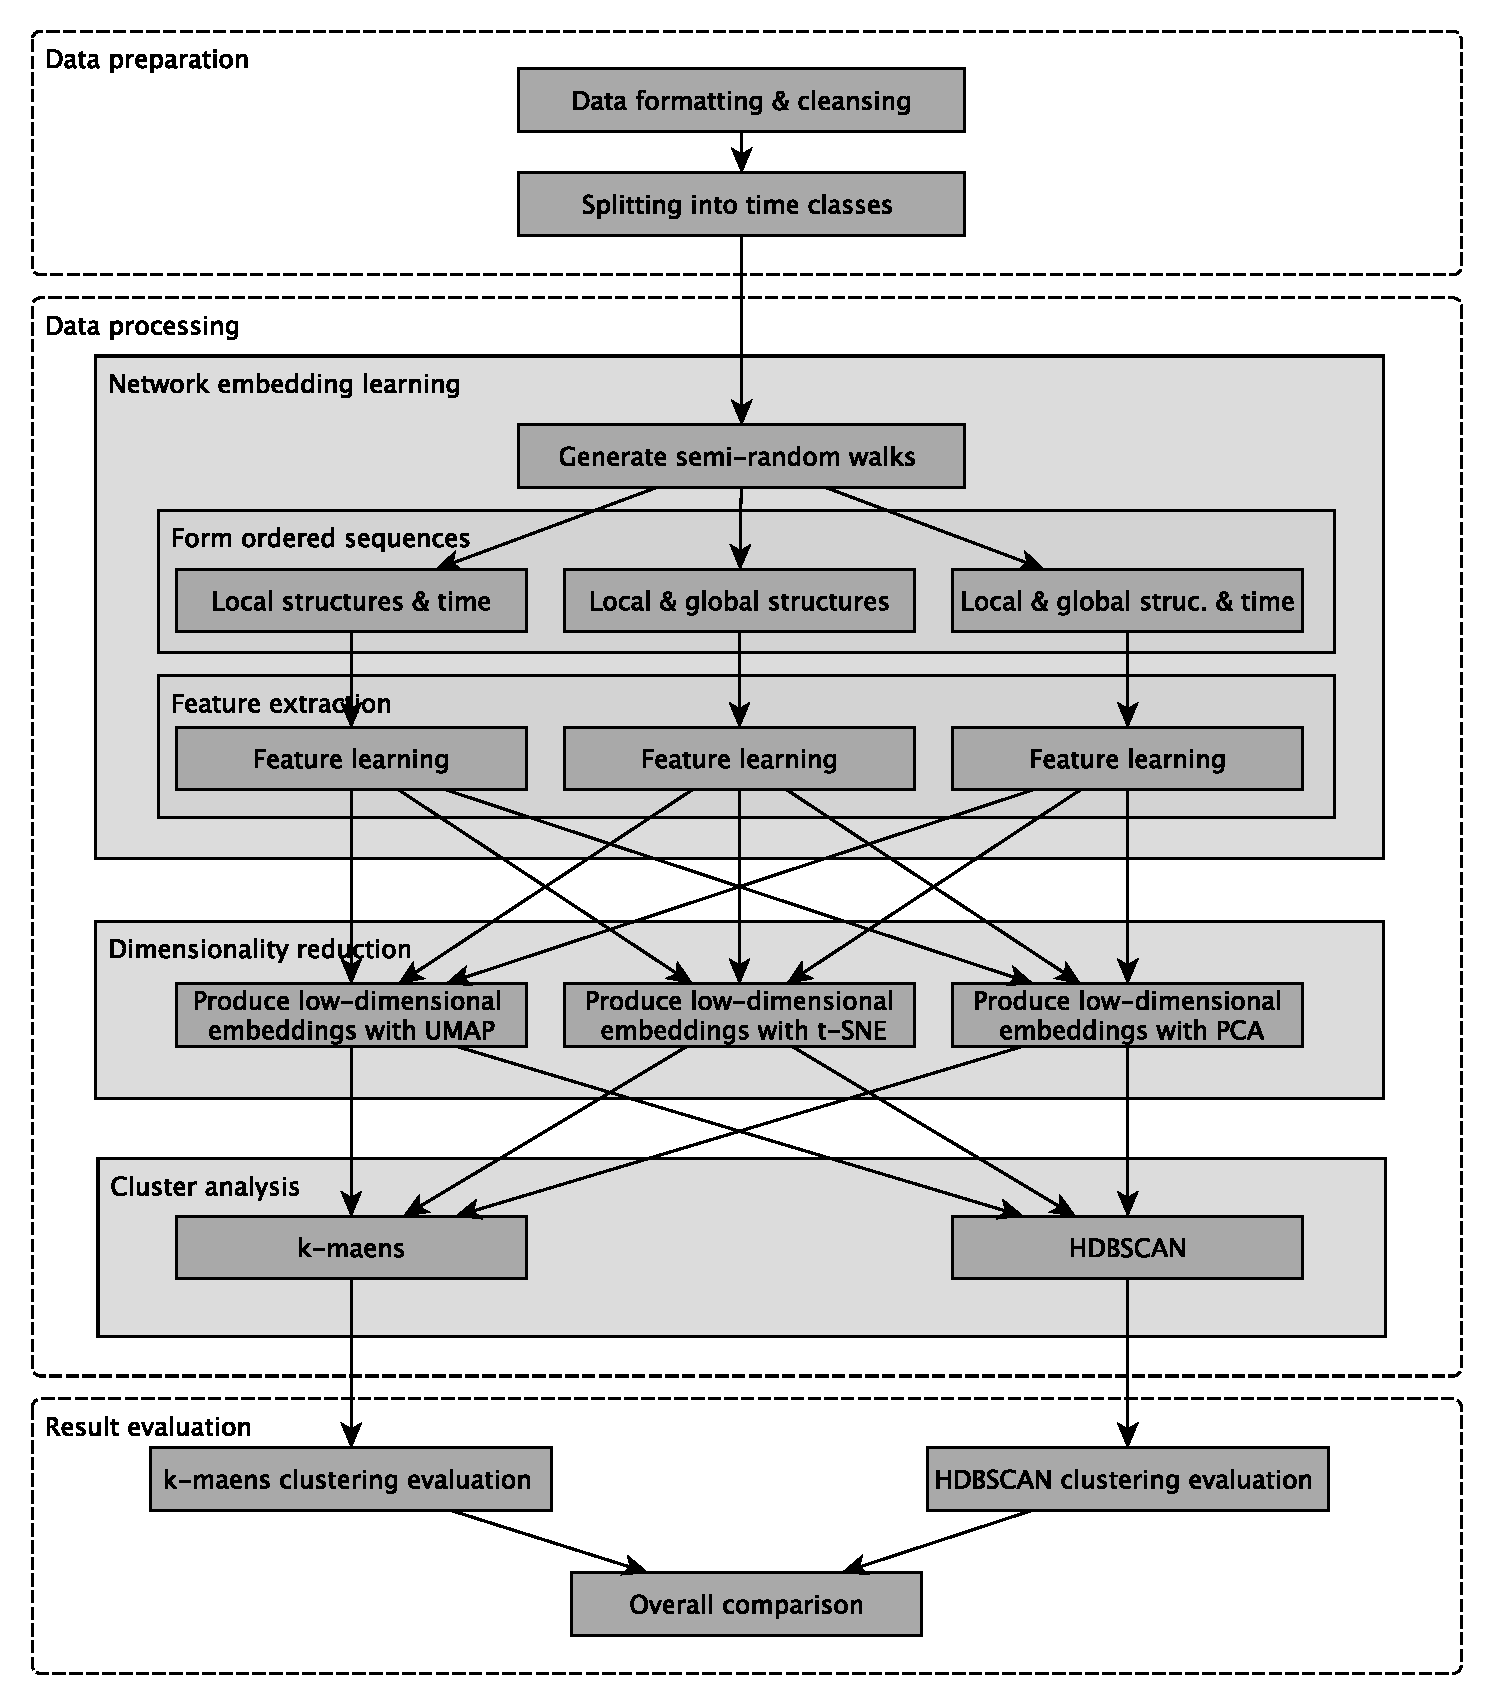
\includegraphics[width=0.67\textwidth]{images/Fig33.pdf}\\
	\caption{The implementation stages of the branched data science pipeline.}
	\label{fig:Fig33}
\end{figure}

The evaluation phase assesses the clustering quality by a set of internal validation measures~\footnote{\textbf{Internal clustering validation measures} - indices which are based on information from the data only and do not consider ground truth labels~\cite{hamalainen2017comparison}}. The set of 8 measures (discussed in~\ref{Concept evaluation}) helps to identify the best data partitioning in terms of compactness, connectedness and separation of clusters. First, the evaluation metrics are used to determine hyperparameters of a clustering, then to compare clustering results from all possible pipeline branches between each other. ~\autoref{fig:Fig33} presents the described overall pipeline divided into implementation stages. The arrows denote data flow along the all possible branches of the pipeline.

\section{Demo application}
\label{Demo application}
A web-based analytics application is developed to demonstrate the application of the concept to artificial data sets. It visualizes the resulting embeddings from the different pipeline's branches interactively. Furthermore, it allows to tune parameters of the unsupervised techniques used on different stages and to observe changes in the results immediately. 

The purpose is to demonstrate the idea by feeding the pipeline with the small artificial data sets, which are not only very fast to process but also exhibit extreme patterns of network structures. Due to these input examples, a user can quickly grasp the intuition behind the developed analytical approach. The set of artificially-generated inputs can be easily extended within the application. At the moment of the thesis delivery there are following predefined data sets:
    \begin{itemize}
        \item random network,
        \item star network,
        \item network of two disconnected star components,
        \item network of two connected star components,
        \item network of two disconnected components of nodes sampled from normal distributions,
        \item network of two disconnected components each sampled as a Watts–Strogatz model graph with edges belonged to 4 different time classes (2 classes per component),
        \item network of two disconnected components each sampled as a Watts–Strogatz model graph with edges belonged to 3 different time classes (1 class per component + 1 class presented in both components),
        \item grid graph model.
    \end{itemize}

From the technical perspective, the application is essentially a web-wrapper around the primary pipeline. It was implemented using Python framework - Dash. Dash is an abstraction built on top of Flask~\footnote{\textbf{Flask} is one of the most popular lightweight Python WSGI application frameworks based on the Jinja template engine and the Werkzeug WSGI toolkit. Source: https://flask.palletsprojects.com} which allows to wrap a user web-interface around a Python analytics script.~\autoref{fig:Fig34} depicts an architecture of the Dash application.

\begin{figure}[!ht]
	\centering
	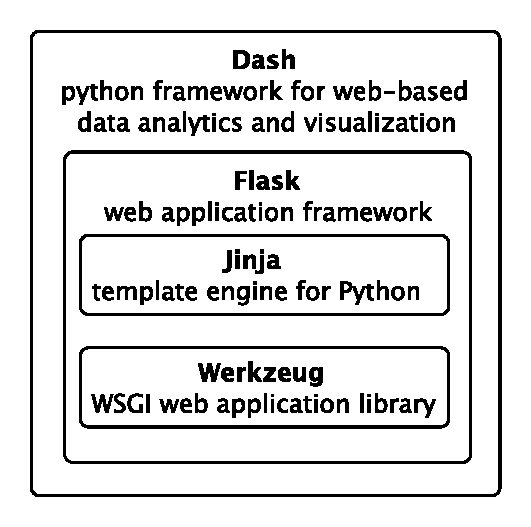
\includegraphics[width=0.35\textwidth]{images/Fig34.pdf}\\
	\caption{Architecture of the Dash application.}
	\label{fig:Fig34}
\end{figure}

The application provides an interactive user-friendly web-interface.~\autoref{fig:Fig35} presents the first screen of the interactive interface. A user can choose the initial parameters of Node2vec framework for feature learning from a selected network. Additionally, user chooses the components for ordered sequences generation (degree and/or time). The location component is chosen by default as it is necessary for Node2vec framework. The application visualizes the reduced embeddings in a 3d space produced by the three dimensionality reduction techniques. It also allows to set hyperparameters for these techniques and observe changes in the outputting visualizations.

\begin{figure}[!ht]
	\centering
	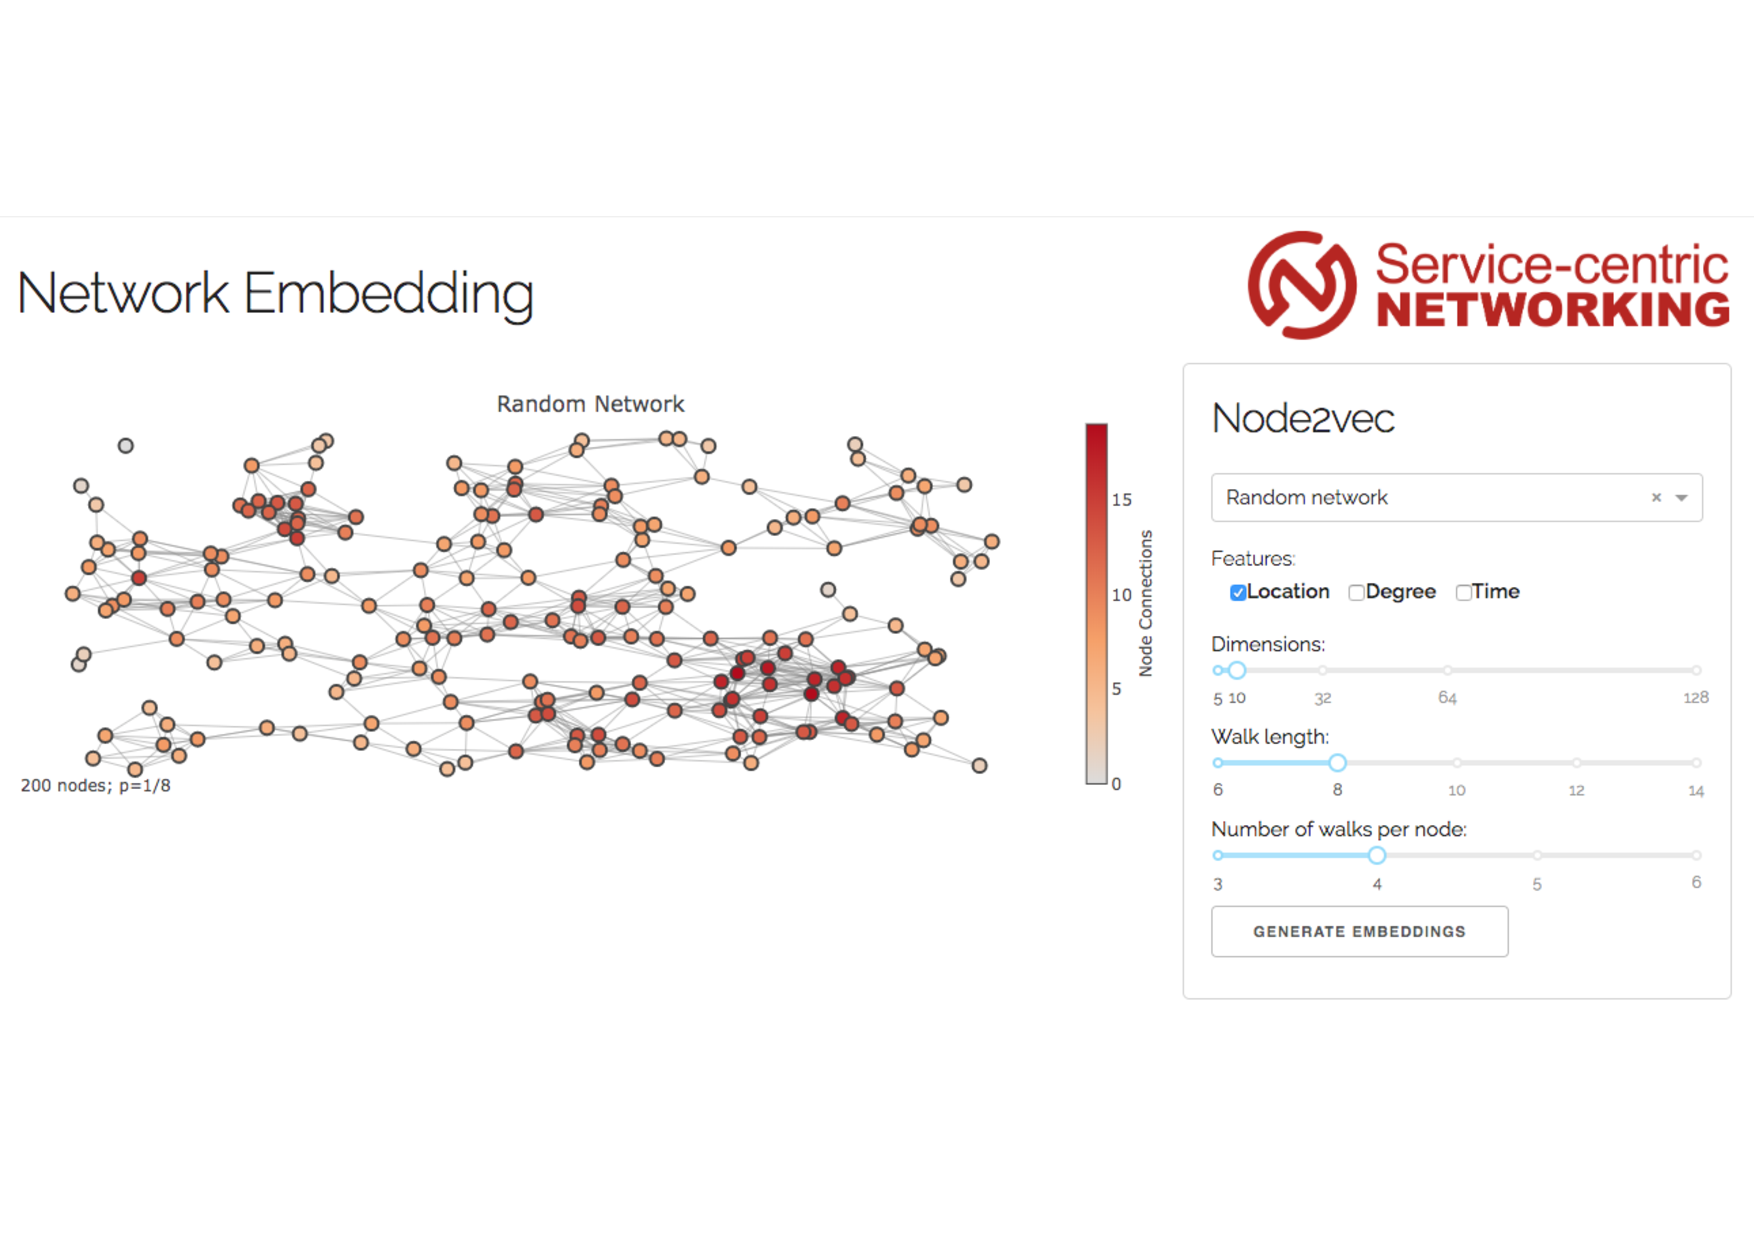
\includegraphics[width=0.65\textwidth]{images/Fig35.pdf}\\
	\caption{First screen web-interface of the application.}
	\label{fig:Fig35}
\end{figure}

\section{Result evaluation}
\label{Result evaluation}

The last stage of the pipeline produces a set of clusters. Thereby the evaluation of the concept boils down to measuring the quality of clustering.

As mentioned in~\ref{Cluster Analysis} there are various clustering techniques for different purposes and types of tasks. The pipeline exploits two very different from each other techniques on the same input data: partitional and density-based clustering. The goodness of clustering is typically measured by internal and external measures. While external validation metrics require ground truth labels, which in the current case is not provided, internal clustering validation metrics consider solely the available outputting clusters.

The evaluation stage of the obtained results on~\autoref{fig:Fig33} exploits a set of internal clustering validation metrics (listed in~\ref{Concept evaluation}). The achieved results from two different clustering techniques are compared separately. It means that outputs of several branches ended in $k$-means clustering will be compared among themselves. The comparison by eight internal validation metrics will highlight the leader among all possible k-means clustering results from the corresponding branches. However, k-means clustering has a well-known weakness in determining the number of clusters. The elbow method resolves this uncertainty by finding the best number of clusters for each particular branch result. The x-axis of the elbow plot described in~\ref{k-means} represents the number of clusters while the y-axis identifies the corresponding within-cluster sum of squares. The "elbow criterion" states to choose the number of clusters at which marginal gain in the within-cluster sum of squares drops and the curve outlines a slight angle. However, it is not always possible to clearly state the number of clusters $k$ from the plot. The set of internal clustering validation metrics facilitates the choice by pointing to a clustering with the best metrics' scores. Once the optimal number of clusters $k$ has been determined, the $k$-means clustering results from two branches compete with each other by achieving the best magnitudes for the eight internal clustering measures.

The second endpoint of the data processing stage on~\autoref{fig:Fig33} is the HDBSCAN clustering. This technique defines a number of clusters automatically by some density-based hiperparameters. A search grid helps to identify the best clustering parameters for each case. The grid considers the most crucial HDBSCAN clustering parameters:
    \begin{itemize}
        \item \textbf{minimum cluster size} - the minimum number of points recognized as a separate cluster,
        \item \textbf{minimum number of samples} - the number of samples in a neighbourhood for a point to be considered a core point (explained on the ~\autoref{fig:Fig23}),
        \item \textbf{alpha} - a distance scaling parameter (increasing alpha will make the clustering more conservative).
    \end{itemize}
Each HDBSCAN clustering result is generated for a different set of hyperparameters, estimated by the set of internal clustering measures, and then compared with other HDBSCAN results.

Finally, the two clustering winning results (one from k-means, one form HDBSCAN) are compared to each other in order to find the best clustering for the original input data.

\section{Deliverables}
The current work comes with the reproducible code of the implementation of the data science pipeline over the concept proposed in chapter~\ref{cha:conceptanddesign}. Additionally, the original financial data set used for the experiments described in the next chapter is attached.

This master thesis is submitted with a storage medium contained the following deliverables:
\begin{enumerate}
    \item Set of Jupyter notebooks written in Python: all data processing stages of the pipeline are implemented in Python 3.7. The notebooks contain all consecutive stages with comments, outputs, and related visualizations. They differ in the components considered for in the automated feature learning framework from networks at the first stage of the pipeline (described in~\ref{Automated Feature Learning Framework}):
    \begin{itemize}
        \item \textbf{Pipeline\_time.ipynb} contains all steps of the pipeline and considers the transactions' time of occurrence in the feature learning process \ref{Time component}.
        \item \textbf{Pipeline\_structures.ipynb} contains all steps of the pipeline and takes into account the global structural component described in the \label{Global structural component} in the feature learning.
        \item \textbf{Pipeline\_time\_structures.ipynb} contains all steps of the pipeline and considers both transactions' time and global structural component derived from a network.
    \end{itemize}
    \item Intermediate computational results of the experiments on the real-world data set:
    \begin{itemize}
        \item \textbf{Embeddings} - set of three files with the embeddings generated from the financial network by the automated feature learning framework (each file for time, global structures, and time-global structures components used for embeddings learning).
        \item \textbf{Labels} - set of three files with arrays of labels: the ids of the nodes whose representations have been learned.
        \item \textbf{K-means clustering results} - set of files with clusters of nodes grouped together as similar in some sense. They result from the branched pipeline using $k$-means clustering.
        \item \textbf{HDBSCAN clustering results} - set of files with clusters of nodes grouped together as similar in some sense. They result from the branched pipeline using HDBSCAN clustering.
    \end{itemize}
    \item Real-world data set of financial transactions between users of the~\href{www.prosper.com} platform. The data set consists of "Source" and "Target" fields which denote the users with the valid prosper account on the platform and "Timestamp" characterising when a "Source" has initiated a transaction to a "Target".
    \item Web-based analytics demo application highlights the main pipeline stages and interactively illustrates the idea by processing artificially-generated basic examples. It allows to tune model's hyperparameters and produces 3d visualizations.
\end{enumerate}

\section{Summary}
This chapter discussed the toolset involved in the development and justified its choice. Here, a reader can find the list of frameworks and packages along with their purposes of usage in the current work. The implementation of the pipeline's stages was discussed in detail. The chapter demonstrated the data flow along the pipeline branches and described the expected result. Additionally, the technical aspects of the demo application were outlined. The chapter explained the evaluation strategy exposed to the achieved results and listed the thesis deliverables.
